% !TEX root = ../main.tex
%

\subsection{勾配を用いた最適化}

ここでは、勾配を用いた最適化アルゴリズムをまとめる。

\begin{algorithm}[tp]
    \caption{勾配による最適化}
    \label{optimization_unconstrained_descent-methods_general-descent-method}
    \begin{algorithmic}
        \Procedure{DescentMethod}{$f, \bm{x}_0$}
            \For{$i = 1,2,\ldots$}
                \State 更新方向 $\bm{d}_i \in \setR^n$ を算出する
                \State 直線探索により更新方向に掛ける係数 $t_i$ を決定する
                \Comment{通常 $f(\bm{x}_{i-1} + t_i \bm{d}_i) < f(\bm{x}_{i-1})$ とする}
                \State $\bm{x}_i \gets \bm{x}_{i-1} + t_i \bm{d}_i$
                \If{終了条件を満たしている}
                    \State \Return $\bm{x}_i$
                \EndIf
            \EndFor
        \EndProcedure
    \end{algorithmic}
\end{algorithm}

勾配を用いた最適化アルゴリズムでは、
一般に
Algorithm \ref{optimization_unconstrained_descent-methods_general-descent-method}
のような手順で反復的に最適化を進めていく。
更新方向の算出方法により、
最急降下法、ニュートン法、共役勾配法のような様々なアルゴリズムが存在する。

\subsubsection{直線探索}

まずは、直線探索の方法をまとめる。
直線探索の方法として、以下のような方法が挙げられる。

\begin{itemize}
    \item 厳密直線探索
    \item Backtracking line search
\end{itemize}

厳密直線探索は、更新後の目的関数の値
$f(\bm{x}_{i-1} + t_i \bm{d}_i)$
が最小となる $t_i$ を探索する。

\begin{algorithm}[tp]
    \caption{Backtracking Line Search \cite[Section 9.2]{Boyd2004}}
    \label{optimization_unconstrained_descent-methods_BacktrackingLineSearch}
    \begin{algorithmic}
        \Procedure{BacktrackingLineSearch}{$f, \bm{x}_{i-1}, \bm{d}_i$}
            \State $t_i \gets 1$
            \While{$f(\bm{x}_{i-1} + t_i \bm{d}_i) > f(\bm{x}_{i-1}) + \alpha t_i \nabla f(\bm{x}_{i-1})^\top \bm{d}_i$}
                \State $t_i \gets \beta t_i$
            \EndWhile
        \EndProcedure
    \end{algorithmic}
\end{algorithm}

\begin{figure}[tp]
    \centering
    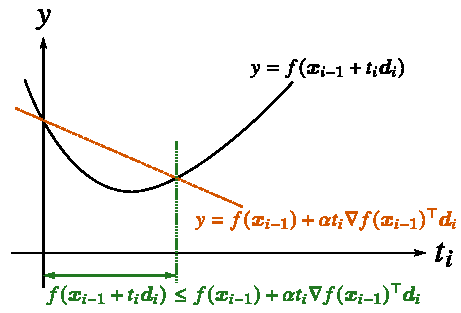
\includegraphics[width=0.7\linewidth]{optimization/Armijo-rule-image.pdf}
    \caption{Armijo の条件(式\eqref{optimization_unconstrained_descent-methods_Armijo-rule})のイメージ}
    \label{optimization_unconstrained_descent-methods_Armijo-rule-image}
\end{figure}

Backtracking Line Search \cite[Section 9.2]{Boyd2004} は
Armijo の条件 \cite[Section 7.5]{Luenberger2003}
\begin{equation}
    f(\bm{x}_{i-1} + t_i \bm{d}_i) \le f(\bm{x}_{i-1}) + \alpha t_i \nabla f(\bm{x}_{i-1})^\top \bm{d}_i
    \label{optimization_unconstrained_descent-methods_Armijo-rule}
\end{equation}
を利用する。
ここで、$\alpha$ は $\alpha \in (0,1)$ を満たす定数であるが、
Backtracking Line Search においては、$\alpha \in (0, 1/2)$ とする
(この場合の条件は Goldstein Test \cite[Section 7.5]{Luenberger2003} と呼ばれる)。
Armijo の条件は、
図\ref{optimization_unconstrained_descent-methods_Armijo-rule-image}のように
十分小さい $t_i$ を選択するための条件となっている。
Backtracking Line Search では、
Algorithm \ref{optimization_unconstrained_descent-methods_BacktrackingLineSearch}
のように
$t_i$ を初期値 1 から $\beta \in (0, 1)$ 倍していき、
式 \eqref{optimization_unconstrained_descent-methods_Armijo-rule} を満たすものを探索する。
一般に、パラメータ $\alpha$, $\beta$ は
$\alpha \in [0.01, 0.3]$, $\beta \in [0.1, 0.8]$ の範囲で設定される
\cite[Section 9.2]{Boyd2004}。
